\chapter{Aufbau \programname}

\section{Architekturbeschreibung}
Im Groben gehalten funktioniert der Daten- und Befehlsfluss im Trufflehog-Entwurf
wie im klassischen MVC, der Presenter aktiviert Services, welche das Model basierend
auf dem empfangenen Netzwerkverkehr verändert und das View aktualisiert sich am Model.
Da viele Threads im Programm parallel durchlaufen aber dennoch kommunizieren müssen,
verlassen wir uns an einigen Stellen auf das \gls{observerpattern} mit einer
Multi-Thread kompatiblen Datenstruktur.\newline
\newline

\section{Paketbeschreibung}

\subsection{command}

Die Kernfunktionalität innerhalb des Programms stellt das \textbf{command Paket}.
Darin befinden sich sowohl die Hierarchie, vorhandene Datenstruktur als auch jede
mögliche Command-Klasse und deren Interface. Vom Prinzip her vergleichbar mit
Runnables.\newline

\begin{figure}[H]
  \centering
  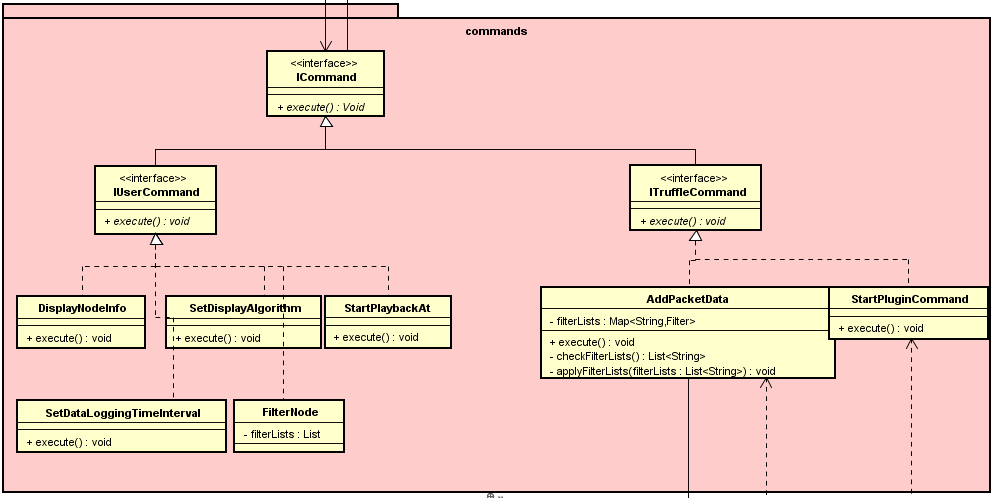
\includegraphics[width=\textwidth]{../diagramimages/commands.png}
  \caption{command Paket}
\end{figure}

Es gibt 2 Hauptarten von Commands, UserCommands für die Verwaltung der
Benutzeroberflächenbefehle, und TruffleCommands für die Methodenaufrufe im
Model-Graph, also die Hauptarbeit am Model. Die Commands machen außerdem den
Hauptteil der Log-Datein und damit der Video-Funktion aus. Mehr dazu im
service-Unterpackage datalogging.

\subsubsection{Command Queue}
Die besagte Datenstruktur, welche beispielsweise der executor besitzt. Es
sind ggf. mehrere tatsächliche Queues vorhanden, was einen Manager verlangt
um nach dem Round-Robin-Prinzip faire Verteilung zu ermöglichen.


\subsection{service}


In unserem Entwurf haben wir uns außerdem dazu entschieden einzelne
durchlaufende Arbeitsschritte in das service Paket auszulagern.\newline

\begin{figure}[H]
  \centering
  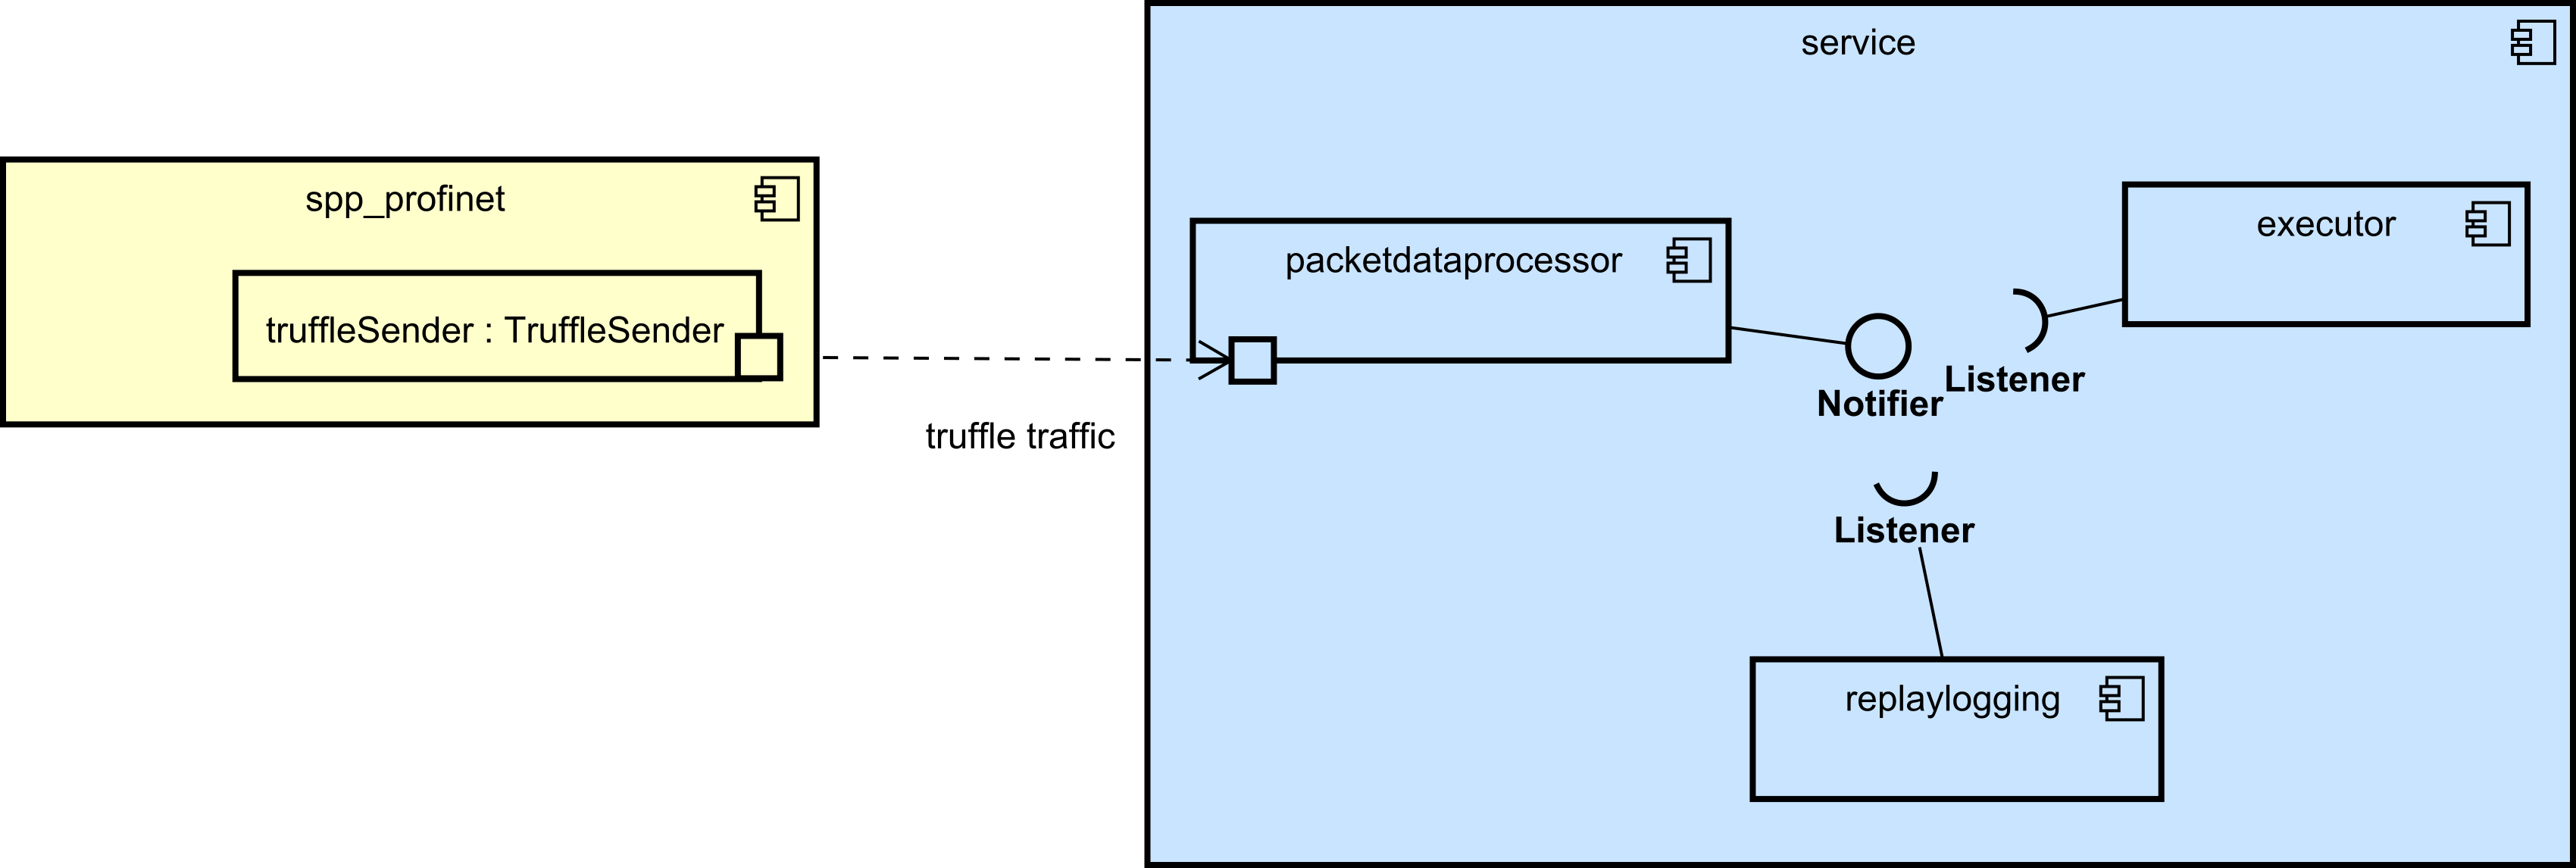
\includegraphics[width=\textwidth]{../diagramimages/service.png}
  \caption{service Paket}
  \medskip
\end{figure}

    \subsubsection{truffleprocessor}
    Der truffleprocessor ist die Empfangsstelle für die von uns in der
    \gls{ipc} benutzen Truffles. Außerdem erzeugt er die später verwendeten
    Commands und benachrichtigt als \gls{notifier}.

    \subsubsection{datalogging}
    Das datalogging kümmert sich um die gesamte gewünschte
    Speicherung/Loggen und, falls implementiert, die Verfügbarkeit der
    Video-Daten. Es speichert sowohl regelmäßige Snapshots des gesamten
    Graphen, als auch einzelne Commands für eine Schrittweise Rückverfolgung
    des Ablaufes.

    \subsubsection{executor}
    Der executor ist das Unterpackage, in welchem die Anwendung bzw.
    Ausführung der Commands stattfindet. Er ist ein \gls{listener} für Commands
    von sowohl dem view-Package als auch dem truffleprocessor.


\subsection{presenter}


Der presenter ist für den Aufbau von \gls{programname}, also das
Initialisieren, Instanziieren und Referenzieren aller Programmelemente zuständig.

\begin{figure}[H]
  \centering
  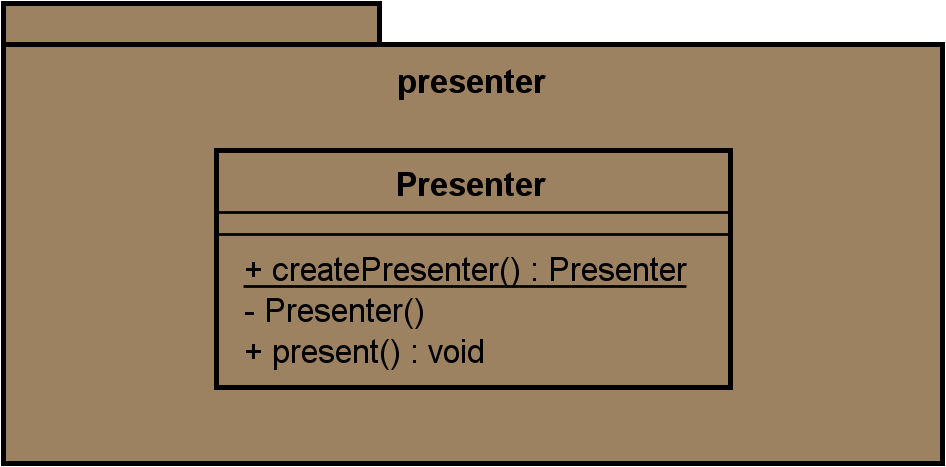
\includegraphics[width=\textwidth]{../diagramimages/presenter.png}
  \caption{presenter Paket}
\end{figure}

Er ist der erste Thread und erzeugt alle weiteren, zum Beispiel einen für jeden
Service. Außerdem liest er aus einer Settings-Datei und stellt das Programm ein.
Das heisst er initialisiert bestimmte Attribute entsprechend. Danach erschöpft
sich die Nützlichkeit des presenter bis zu einem neuen Programmstart.


\subsection{util}


Unsere Variante des \gls{observerpattern}s.

\begin{figure}[H]
  \centering
  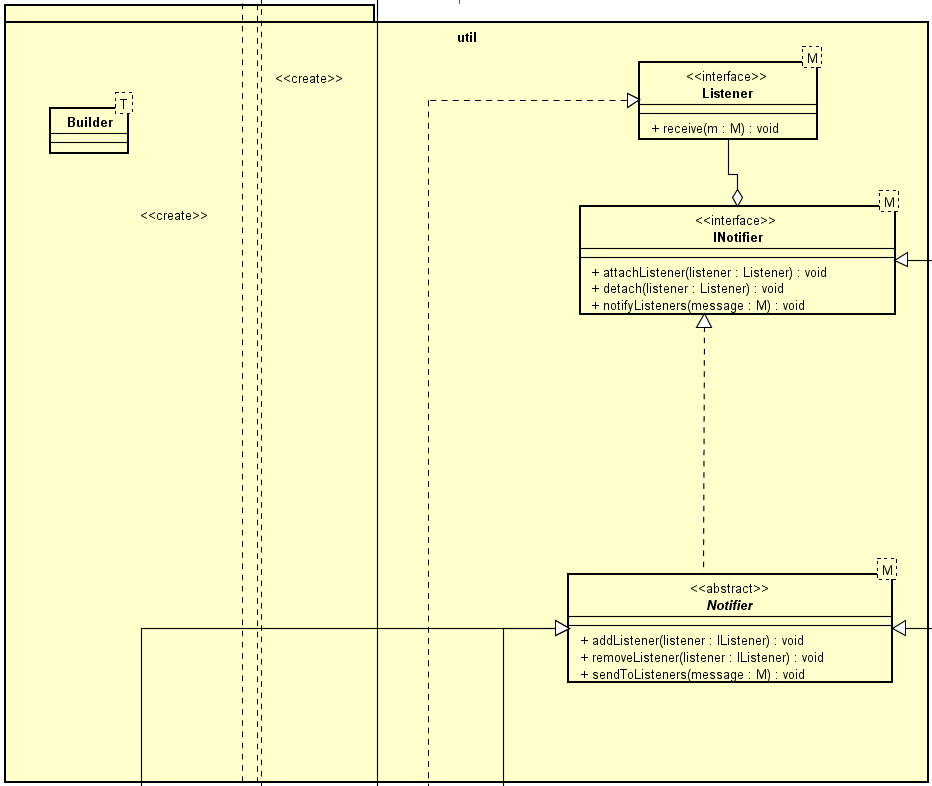
\includegraphics[width=\textwidth]{../diagramimages/util.png}
  \caption{util Paket}
\end{figure}

Da wir sowohl Interfaces als auch Klassen bzw. abstrakte Klassen als
\gls{notifier} haben, kommen wir nicht um eine Modifizierung des klassischen
\gls{observerpattern} herum. Nun haben wir die Möglichkeit sowohl ein
\gls{notifier}-Interface zu erweitern als auch eine abstrakte
\gls{notifier}-Klasse zu beerben. Der \gls{listener} funktioniert genau wie ein
Observer.


\subsection{model}


Die Hauptdatenstruktur von \gls{programname}: das model Paket.

\begin{figure}[H]
  \centering
  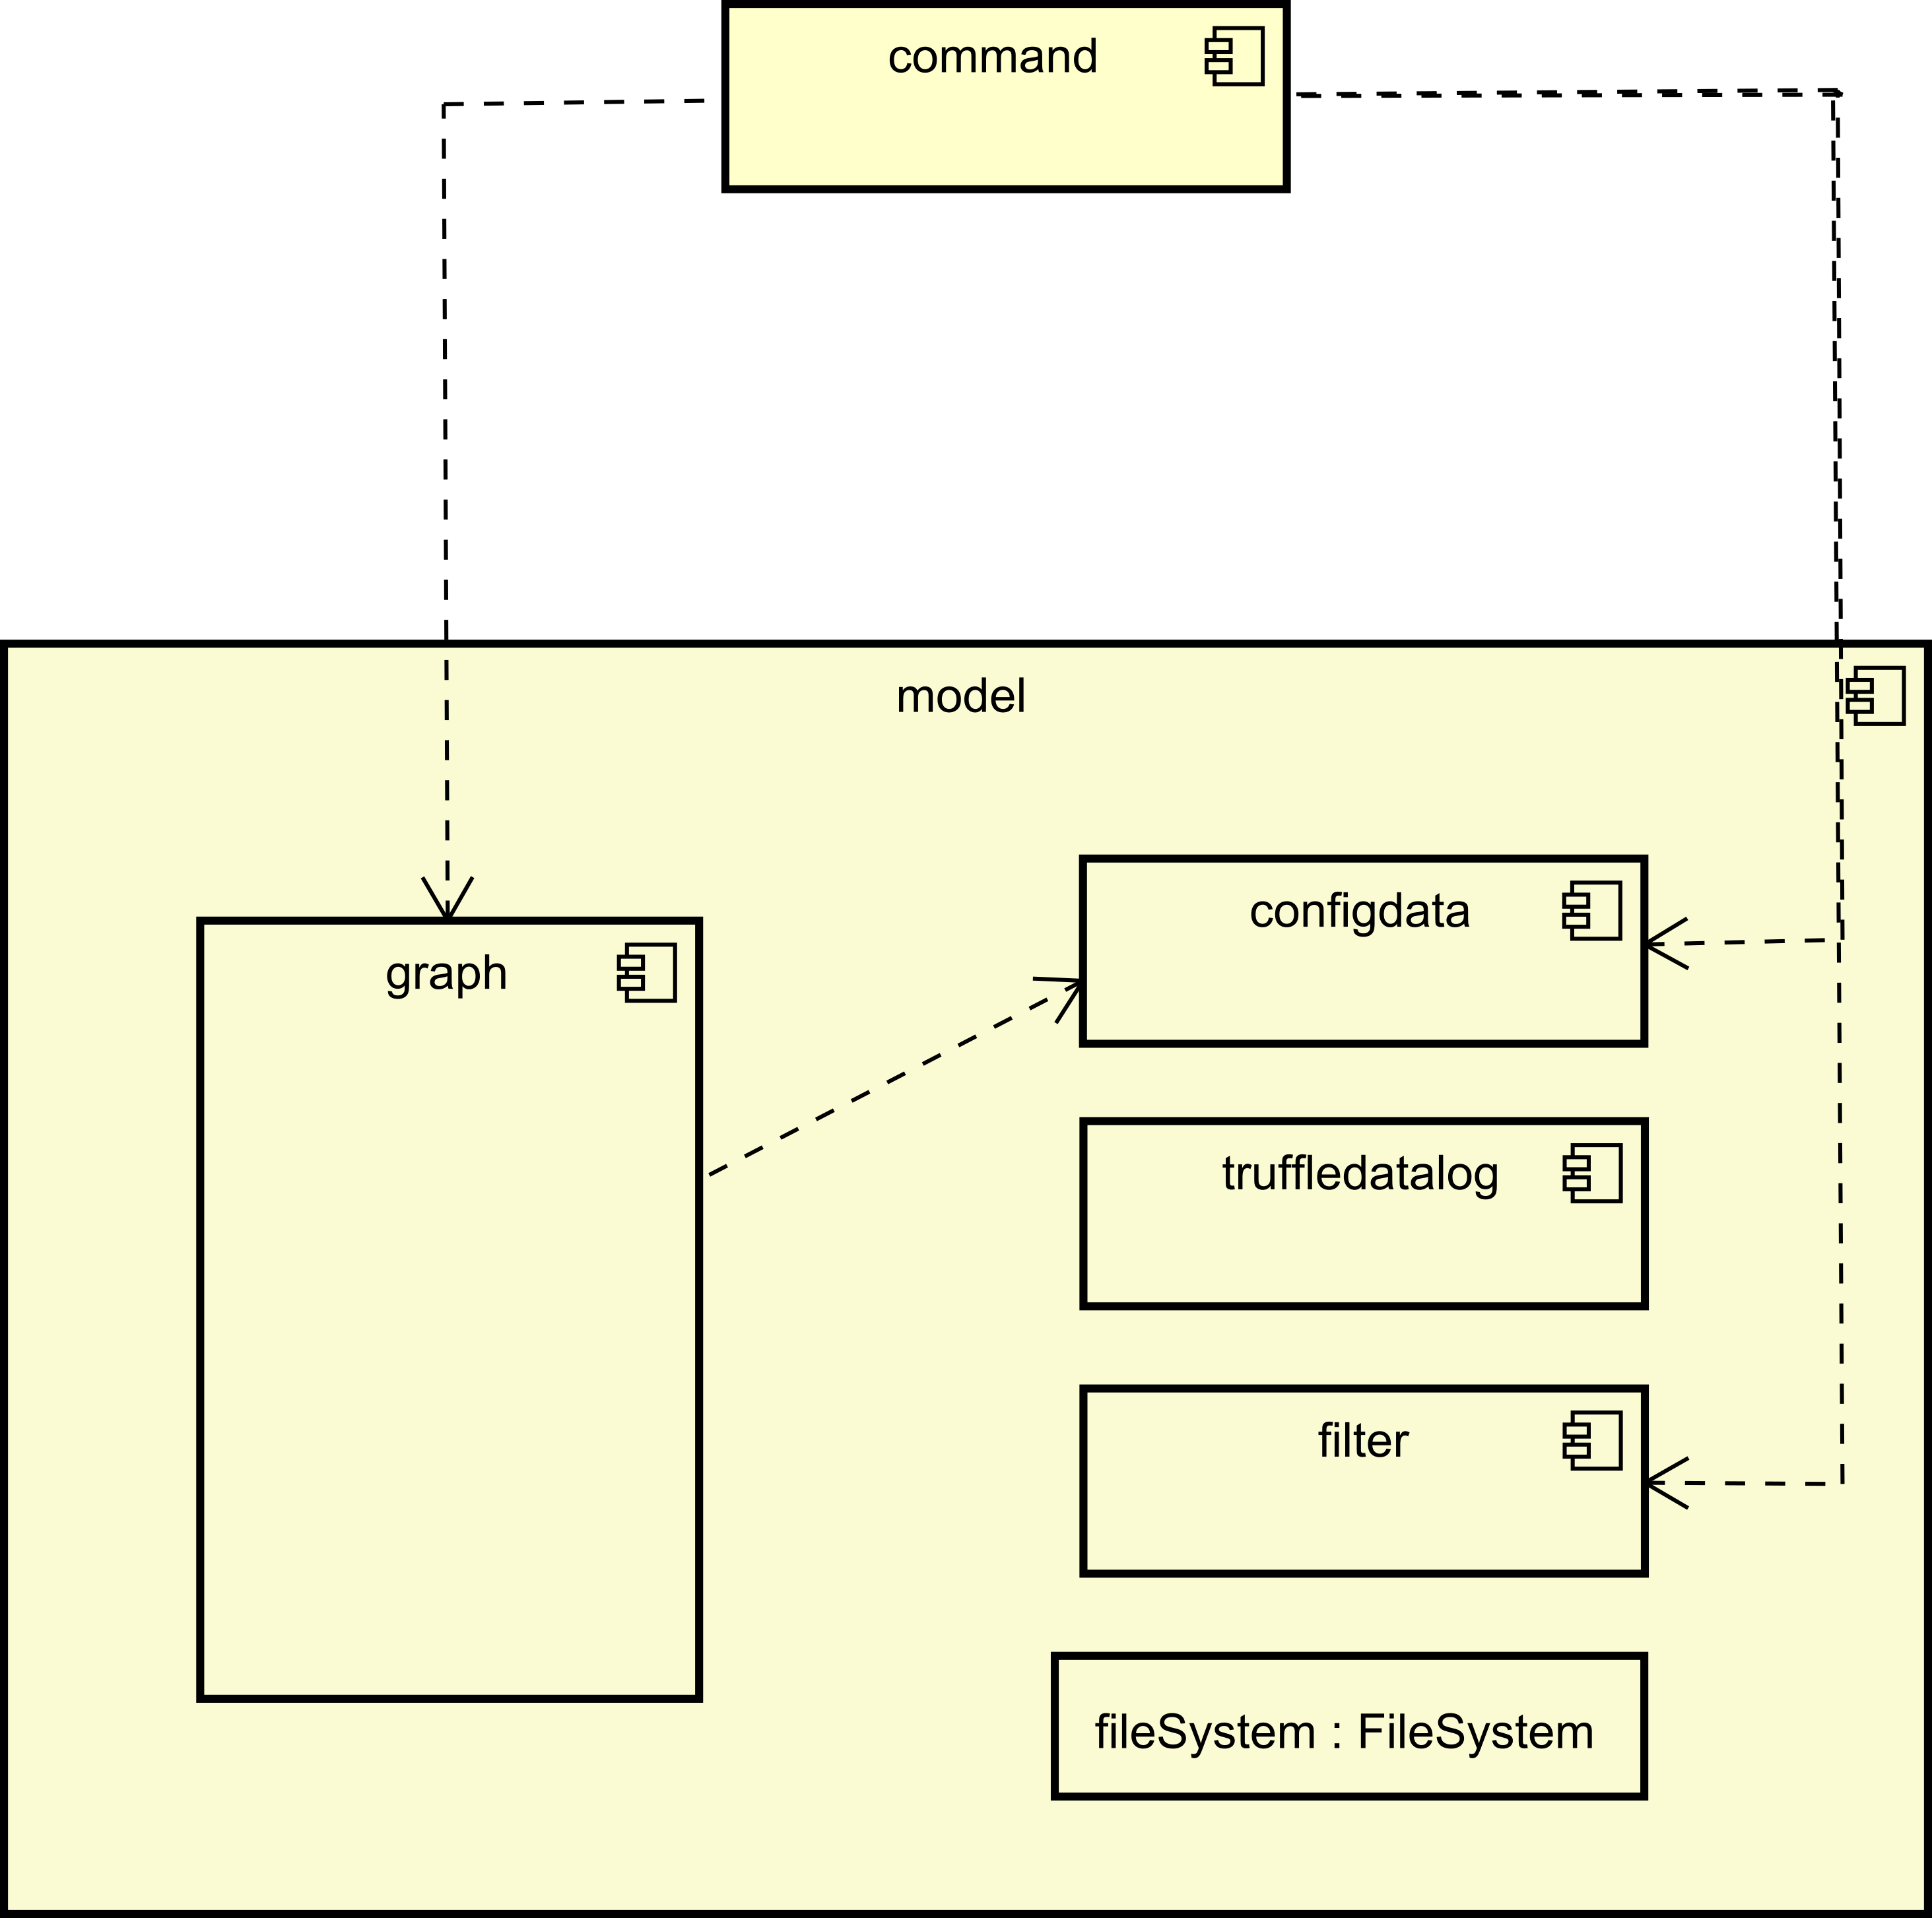
\includegraphics[width=\textwidth]{../diagramimages/model.png}
  \caption{model Paket}
\end{figure}

    \subsubsection{graph}

    \subsubsection{filter}

    \subsubsection{settingsdata}

    \subsubsection{graphlog}


\subsection{view}

\subsection{interactors}
